\documentclass[resume]{subfiles}


\begin{document}
    \section{Interpolation}
    $$\boxed{n+1\ \text{points}}$$
    \subsection{Polynôme d'interpolation de Lagrange avec 3+1 points}
    $$l_{\textcolor{OrangeRed}{0}}(x)=\textcolor{RoyalBlue}{\lambda}_{\textcolor{OrangeRed}{0}}(x_{\ }-x_{\textcolor{ForestGreen}{1}})(x_{\ }-x_{\textcolor{ForestGreen}{2}})(x_{\ }-x_{\textcolor{ForestGreen}{3}})$$
    $$\textcolor{RoyalBlue}{\lambda}_{\textcolor{OrangeRed}{0}}=\frac{1}{(x_{\textcolor{OrangeRed}{0}}-x_{\textcolor{ForestGreen}{1}})(x_{\textcolor{OrangeRed}{0}}-x_{\textcolor{ForestGreen}{2}})(x_{\textcolor{OrangeRed}{0}}-x_{\textcolor{ForestGreen}{3}})}$$
    $$l_{\textcolor{OrangeRed}{1}}(x)=\textcolor{RoyalBlue}{\lambda}_{\textcolor{OrangeRed}{1}}(x_{\ }-x_{\textcolor{ForestGreen}{0}})(x_{\ }-x_{\textcolor{ForestGreen}{2}})(x_{\ }-x_{\textcolor{ForestGreen}{3}})$$
    $$\textcolor{RoyalBlue}{\lambda}_{\textcolor{OrangeRed}{1}}=\frac{1}{(x_{\textcolor{OrangeRed}{1}}-x_{\textcolor{ForestGreen}{0}})(x_{\textcolor{OrangeRed}{1}}-x_{\textcolor{ForestGreen}{2}})(x_{\textcolor{OrangeRed}{1}}-x_{\textcolor{ForestGreen}{3}})}$$
    $$l_{\textcolor{OrangeRed}{2}}(x)=\textcolor{RoyalBlue}{\lambda}_{\textcolor{OrangeRed}{2}}(x_{\ }-x_{\textcolor{ForestGreen}{0}})(x_{\ }-x_{\textcolor{ForestGreen}{1}})(x_{\ }-x_{\textcolor{ForestGreen}{3}})$$
    $$\textcolor{RoyalBlue}{\lambda}_{\textcolor{OrangeRed}{2}}=\frac{1}{(x_{\textcolor{OrangeRed}{2}}-x_{\textcolor{ForestGreen}{0}})(x_{\textcolor{OrangeRed}{2}}-x_{\textcolor{ForestGreen}{1}})(x_{\textcolor{OrangeRed}{2}}-x_{\textcolor{ForestGreen}{3}})}$$
    $$l_{\textcolor{OrangeRed}{3}}(x)=\textcolor{RoyalBlue}{\lambda}_{\textcolor{OrangeRed}{3}}(x_{\ }-x_{\textcolor{ForestGreen}{0}})(x_{\ }-x_{\textcolor{ForestGreen}{1}})(x_{\ }-x_{\textcolor{ForestGreen}{2}})$$
    $$\textcolor{RoyalBlue}{\lambda}_{\textcolor{OrangeRed}{3}}=\frac{1}{(x_{\textcolor{OrangeRed}{3}}-x_{\textcolor{ForestGreen}{0}})(x_{\textcolor{OrangeRed}{3}}-x_{\textcolor{ForestGreen}{1}})(x_{\textcolor{OrangeRed}{3}}-x_{\textcolor{ForestGreen}{2}})}$$
    \paragraph{Forme 1}
    $$p_3(x)=y_0l_0(x)+y_1l_1(x)+y_2l_2(x)+y_3l_3(x)$$
    \paragraph{Forme 2}
    \begin{multline*}
    p_3(x)=(x-x_0)(x-x_1)(x-x_2)(x-x_3)\\ \cdot\big(y_0\mu_0+y_1\mu_1+y_2\mu_2+y_3\mu_3\big)    
    \end{multline*}
    $$\mu_i=\frac{\lambda_i}{x-x_i}$$
    Forme barycentrique :
    $$p_3(x)=\frac{y_0\mu_0+y_1\mu_1+y_2\mu_2+y_3\mu_3}{\mu_0+\mu_1+\mu_2+\mu_3}$$
    \paragraph{Forme 3 (un peu plus simple à écrire)}
\begin{multline*}
p_2(x)=y_0\frac{(x-x_1)(x-x_2)}{(x_0-x_1)(x_0-x_2)}+\\y_1\frac{(x-x_0)(x-x_2)}{(x_1-x_0)(x_1-x_2)}+y_2\frac{(x-x_0)(x-x_1)}{(x_2-x_0)(x_2-x_1)}
\end{multline*}
    
    \subsection{Polynôme d'interpolation de newton}
    \begin{multline*}
    p_3(x)=c_0+c_1(x-x_0) +c_2(x-x_0)(x-x_1)\\ +c_3(x-x_0)(x-x_1)(x-x_2)
    \end{multline*}
    \begin{figure}[H]
        \centering
        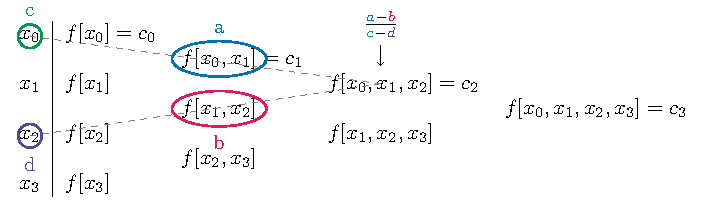
\includegraphics[width=\columnwidth]{drwg_3.pdf}
    \end{figure}
    Possible de rajouter une ligne en dessous du tableau
    
    \subsection{Évaluation}
    On utilise le schéma de Horner
    \begin{figure}[H]
        \centering
        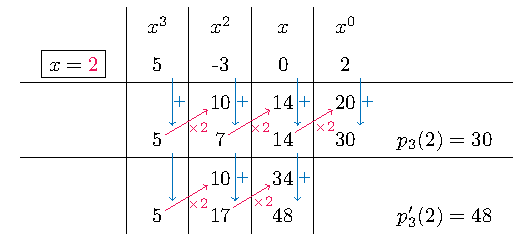
\includegraphics[width=0.8\columnwidth]{drwg_4.pdf}
    \end{figure}
    Après la première dérivée, il faudra appliquer un facteur
    $$\frac{P_n^{(k)}(x_i)}{k!}$$
    \subsection{Erreur}
    Ordre 1 (2 points)
    $$\abs{f(x)-p_1(x)}\leq \frac{1}{8}M_2h^2$$
    Ordre 2 (3 points)
    $$\abs{f(x)-p_2(x)}\leq \frac{\sqrt{3}}{27}M_3h^3$$
    Ordre 3 (4 points)
    $$\begin{cases}
        \abs{f(x)-p_3(x)}\leq \frac{3}{128}M_4h^4 & x\in[x_1,x_2]\\
        \abs{f(x)-p_3(x)}\leq \frac{1}{24}M_4h^4  & x\in[x_0,x_1] \cup [x_2,x_3]
    \end{cases}$$
    Avec
    $$M_{k}=\max_{\zeta\in[a,b]}\abs{f^{(k)}(\zeta)}$$
    L'utilisation des abscisses de Chebychev permettent de minimiser l'erreur avec un nombre de points donnés sur un intervalle donné



\end{document}  